% !TEX root = ../main.tex

%%--------------------------------------------------------------------------
%% ARCHITECTURAL DESIGN
%%--------------------------------------------------------------------------



\chapter{Architecture}
\label{architectural_design}

In this chapter I present what will be the main architecture of the system: it will be composed by a back-end an a front-end.


	\section{Back-end}
	The Back-end will be hosted on a Paas (Google App Engine) and will represent the core functionalities of Pomasana exposing a set of RESTful API; these API will be public and so open to third-party developers so that they will be able to develop applications on any type of platform. The Back-end will communicate with the Asana API and will also offer the authentication functionalities needed to access the system.

	\section{Front-end}
	The front-end will be also hosted on another Paas as Heroku and will be a webapp developed in Javascript; it will take advantage of the features offered by the Pomasana REST API making them accessible to the final users.



		\begin{figure}[h!]
		  \centering
		    \centering{%
		      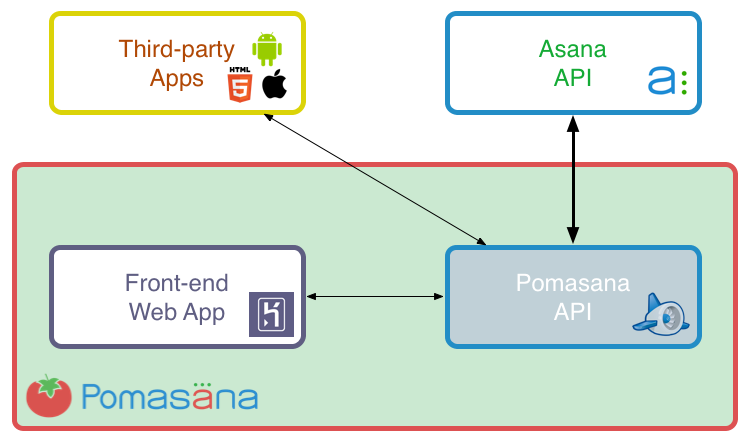
\includegraphics[width=1\textwidth]{arch.png}}
		  \caption{Main Architecture}
		\end{figure}
